\documentclass[a4paper,12pt]{article}
\usepackage[a4paper,top=1.3cm,bottom=2cm,left=1.5cm,right=1.5cm,marginparwidth=0.75cm]{geometry}
\usepackage{cmap}
\usepackage{mathtext}
\usepackage[T2A]{fontenc}
\usepackage[utf8]{inputenc}
\usepackage[english,russian]{babel}
\usepackage{siunitx}
\usepackage{enumitem}
\usepackage{placeins}

\usepackage{graphicx}
\usepackage{subcaption}
\usepackage{amsmath}

\usepackage{wrapfig}
\usepackage{tabularx}
\usepackage{multirow}

\usepackage{hyperref}
\usepackage[rgb]{xcolor}
\hypersetup{colorlinks=true,urlcolor=blue}
\usepackage{siunitx}
\usepackage{amsmath,amsfonts,amssymb,amsthm,mathtools}
\usepackage{mathtools}
\usepackage{icomma}
\mathtoolsset{showonlyrefs=false}
\usepackage{euscript}
\usepackage{mathrsfs}
\DeclareMathOperator{\sgn}{\mathop{sgn}}
\newcommand*{\hm}[1]{#1\nobreak\discretionary{}
{\hbox{$\mathsurround=0pt #1$}}{}}

\newcommand\labname{Экспериментальная проверка закона Видемана-Франца}
\newcommand\labnumber{11.8}

\author{Макаров Лев Евгеньевич}
\title{Лабораторная работа №\labnumber\\\labname}
\date{\today}

\makeatletter
\AddEnumerateCounter{\asbuk}{\russian@asbuk@alph}{щ}
\makeatother

\begin{document}

\begin{titlepage}
    \begin{center}
        {\large МОСКОВСКИЙ ФИЗИКО-ТЕХНИЧЕСКИЙ ИНСТИТУТ (НАЦИОНАЛЬНЫЙ ИССЛЕДОВАТЕЛЬСКИЙ УНИВЕРСИТЕТ)}
    \end{center}
    \begin{center}
        {\large Физтех-школа фотоники, электроники и молекулярной физики}
    \end{center}

    \vspace{4.5cm}
    {\huge
        \begin{center}
            {\bf Отчёт о выполнении лабораторной работы \labnumber}\\
            \labname
        \end{center}
    }
    \vspace{2cm}
    \begin{flushright}
        {\LARGE Автор:\\ Макаров Лев Евгеньевич\\
        \vspace{0.2cm}
        Б04-306}
    \end{flushright}
    \vspace{8cm}
    \begin{center}
        Долгопрудный 2026
    \end{center}
\end{titlepage}

\section{Введение}

\textbf{Цель работы:}
\begin{enumerate}
    \item экспериментально проверить закон Видемана-Франца;
    \item измерить электрическое сопротивление и тепловое сопротивление одного и того же участка металлического образца;
    \item определить постоянную Лоренца для исследуемого образца и сравнить ее с теоретическим и табличными значениями.
\end{enumerate}

\textbf{В работе используются:} экспериментальная ячейка с металлическим образцом и компенсирующим экраном, два источника постоянного тока INSTEK GPR30H10D, вольтметры В7-78/1, вольтметр В7-38, медь-константановые термопары.

\section{Теоретические сведения}

Электроны в металле можно рассматривать как вырожденный ферми-газ. При $T = 0$ заполнены все состояния с волновым вектором меньше некоторого $k_F$, а поверхность, отделяющая заполненные состояния от свободных, называется поверхностью Ферми. Фермиевский волновой вектор определяется из условия заполнения состояний

\begin{equation}
    k_F = \sqrt[3]{3 \pi^2 n},
\end{equation}

а энергия Ферми в модели почти свободных электронов равна

\begin{equation}
    E_F = \frac{\hbar^2 k_F^2}{2m^*}.
\end{equation}

Для нормальных металлов $E_F \sim 1~\text{эВ}$, поэтому при комнатной температуре $k_{\text{Б}}T \ll E_F$. В тепловых процессах участвуют только электроны вблизи поверхности Ферми. Теплоёмкость вырожденного электронного газа оказывается пропорциональной температуре:

\begin{equation}
    C = \frac{\pi^2}{2} N k_{\text{Б}} \frac{k_{\text{Б}}T}{E_F}.
\end{equation}

Коэффициент теплопроводности электронного газа можно оценить как

\begin{equation}
    \kappa = \frac{1}{3} n c V_F^2 \tau_{\text{th}},
\end{equation}

где $c$ --- теплоёмкость на электрон, $V_F$ --- скорость электронов на поверхности Ферми, $\tau_{\text{th}}$ --- время релаксации для переноса тепла. После подстановки теплоёмкости получаем

\begin{equation}
    \kappa = \frac{\pi^2 n k_{\text{Б}}^2 T}{3m^*}\tau_{\text{th}}.
\end{equation}

Проводимость электронного газа в той же модели выражается через время релаксации импульса $\tau_e$:

\begin{equation}
    \sigma = \frac{e^2 n \tau_e}{m^*}.
\end{equation}

Если процессы рассеяния одинаково ограничивают перенос заряда и тепла, то $\tau_{\text{th}} = \tau_e$. Тогда отношение $\kappa / \sigma T$ не зависит от параметров материала:

\begin{equation}
    L = \frac{\kappa}{\sigma T} =
    \frac{\pi^2 k_{\text{Б}}^2}{3e^2}
    = 2{,}44 \cdot 10^{-8}~\frac{\text{Вт}\cdot\text{Ом}}{\text{К}^2}.
    \label{eq:L-theory}
\end{equation}

Это соотношение называется законом Видемана-Франца, а величина $L$ --- постоянной Лоренца.

\section{Экспериментальная установка}

В работе используется металлический стержень, закреплённый в экспериментальной ячейке. На одном конце стержня установлен нагреватель, а между двумя измерительными точками измеряются как падение напряжения при пропускании тока, так и перепад температур. Это позволяет определять электрические и тепловые свойства одного и того же участка образца.

Сопротивление участка образца измеряется четырёхконтактной схемой. Через образец пропускается ток $I$, а вольтметром измеряется падение напряжения $U$ между потенциометрическими контактами. Так как ток через вольтметр практически не течёт, сопротивления токоподводящих контактов не входят в измеряемое падение напряжения.

При измерении теплопроводности образец окружён коаксиальным экраном. Мощность нагрева экрана подбирается так, чтобы термоЭДС между горячими концами образца и экрана обращалась в ноль. В таком режиме радиального потока тепла между образцом и экраном практически нет.

Для участка образца длиной $l$ и площадью поперечного сечения $S$ имеем

\begin{equation}
    R = \frac{1}{\sigma}\frac{l}{S},
\end{equation}

а перепад температур при выделении мощности $P$:

\begin{equation}
    \frac{P}{S} = \kappa \frac{\Delta T}{l}.
\end{equation}

Отсюда для постоянной Лоренца

\begin{equation}
    L = \frac{\kappa}{\sigma T} =
    \frac{PR}{\Delta T}\frac{1}{T}.
\end{equation}

Если зависимость перепада температур от мощности записать как

\begin{equation}
    \Delta T = A P + T_{\varepsilon},
    \label{eq:deltaT-P}
\end{equation}

то для дальнейшей обработки удобно пользоваться формулой

\begin{equation}
    L = \frac{R}{AT}.
    \label{eq:L}
\end{equation}

\section{Результаты измерений и обработка данных}

\subsection*{Измерение ВАХ образца}

Снимем ВАХ образца в диапазоне токов от $-1$ А до $1$ А. Результаты измерений приведены в таблице \ref{tab:vah}. Напряжение измерялось в мВ.

\begin{table}[h]
    \centering
    \small
    \caption{Измеренная ВАХ образца}
    \label{tab:vah}
    \begin{tabular}{|r|r|r||r|r|r|}
        \hline
        № & $I$, А & $U$, мВ & № & $I$, А & $U$, мВ \\
        \hline
         1 & -1.0 & -0.134 & 12 &  0.1 &  0.017 \\
         2 & -0.9 & -0.120 & 13 &  0.2 &  0.030 \\
         3 & -0.8 & -0.106 & 14 &  0.3 &  0.045 \\
         4 & -0.7 & -0.093 & 15 &  0.4 &  0.058 \\
         5 & -0.6 & -0.079 & 16 &  0.5 &  0.072 \\
         6 & -0.5 & -0.065 & 17 &  0.6 &  0.086 \\
         7 & -0.4 & -0.051 & 18 &  0.7 &  0.100 \\
         8 & -0.3 & -0.038 & 19 &  0.8 &  0.114 \\
         9 & -0.2 & -0.024 & 20 &  0.9 &  0.128 \\
        10 & -0.1 & -0.010 & 21 &  1.0 &  0.142 \\
        11 &  0.0 & -0.002 &    &      &        \\
        \hline
    \end{tabular}
\end{table}

Из-за сдвига нуля вольтметра и паразитных термоЭДС ВАХ может не проходить через начало координат, поэтому аппроксимируем зависимость выражением

\begin{equation}
    U(I) = U_0 + R I.
    \label{eq:vah}
\end{equation}

Для коэффициентов получено

\begin{equation}
    R = (1{,}376 \pm 0{,}005)\cdot 10^{-4}~\text{Ом}, \qquad
    U_0 = (3{,}3 \pm 0{,}3)\cdot 10^{-6}~\text{В}.
\end{equation}

График ВАХ и линейной аппроксимации приведён на рис. \ref{pic:vah}.

\begin{figure}[h]
    \centering
    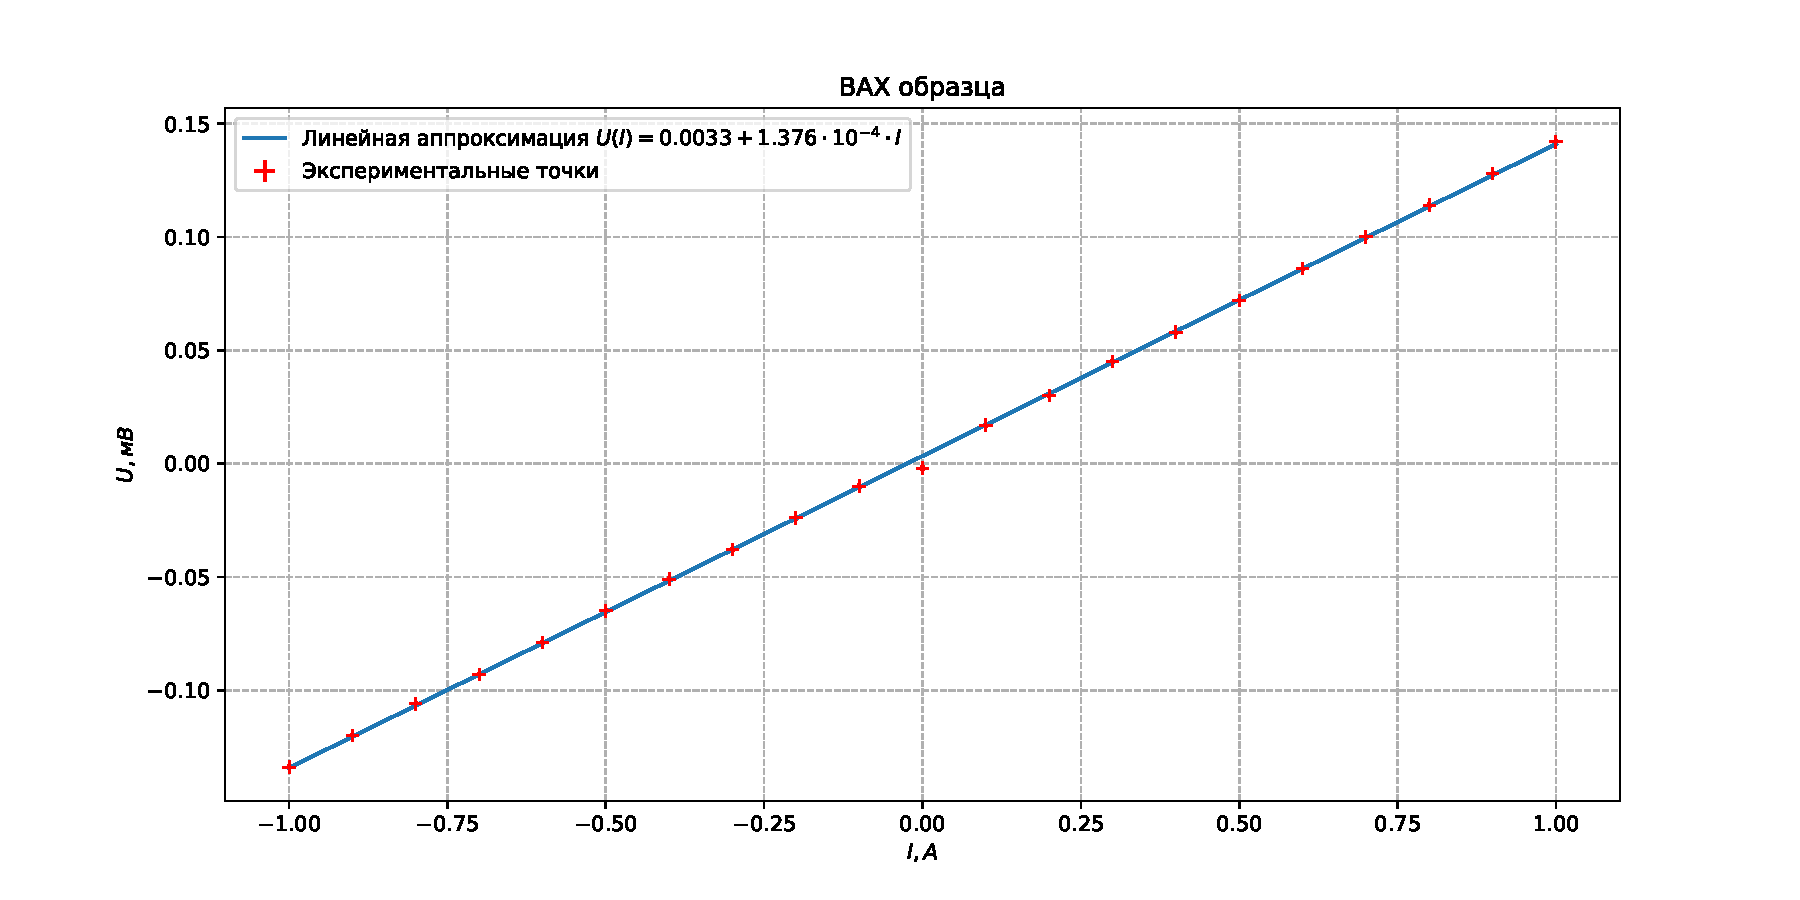
\includegraphics[width=0.8\textwidth]{pictures/graph_vah.pdf}
    \caption{ВАХ образца и линейная аппроксимация}
    \label{pic:vah}
\end{figure}

\subsection*{Измерение теплового сопротивления}

Для разных токов нагревателя образца измерялись напряжение на нагревателе, термоЭДС термопары образца и время установления равновесия. Мощность нагревателя вычислялась как

\begin{equation}
    P = U_N I_N,
\end{equation}

а погрешность мощности:

\begin{equation}
    \sigma_P = \sqrt{I_N^2 \sigma_{U_N}^2 + U_N^2 \sigma_{I_N}^2}.
\end{equation}

Для медь-константановой термопары при комнатной температуре использовалась чувствительность

\begin{equation}
    \alpha = 43~\frac{\text{мкВ}}{\text{К}},
\end{equation}

поэтому при измерении $V$ в мВ

\begin{equation}
    \Delta T = \frac{1000 V}{\alpha}, \qquad
    \sigma_{\Delta T} = \frac{1000\sigma_V}{\alpha}.
\end{equation}

Результаты измерений приведены в таблице \ref{tab:thermo}. Отдельно была исключена точка при $I_N = 0{,}300$ А, так как равновесие устанавливалось только $150$ с и она заметно выпадала из линейной зависимости.

\begin{table}[h]
    \centering
    \small
    \caption{Измерение зависимости $\Delta T(P)$}
    \label{tab:thermo}
    \begin{tabular}{|r|r|r|r|r|r|r|}
        \hline
        № & $U_N$, В & $I_N$, А & $P$, Вт & $V$, мВ & $\Delta T$, К & $t$, с \\
        \hline
        1 & 2.6040 & 0.203 & 0.5286 & 0.310 &  7.21 & 300 \\
        2 & 3.2300 & 0.250 & 0.8075 & 0.501 & 11.65 & 300 \\
        3 & 2.2530 & 0.175 & 0.3943 & 0.277 &  6.44 & 720 \\
        4 & 1.9541 & 0.150 & 0.2931 & 0.199 &  4.63 & 600 \\
        5 & 1.6012 & 0.125 & 0.2002 & 0.136 &  3.16 & 720 \\
        6 & 1.2855 & 0.100 & 0.1286 & 0.088 &  2.05 & 780 \\
        7 & 0.9638 & 0.075 & 0.0723 & 0.054 &  1.26 & 600 \\
        8 & 2.8820 & 0.225 & 0.6485 & 0.389 &  9.05 & 780 \\
        \hline
        выбр. & 3.8570 & 0.300 & 1.1571 & 0.477 & 11.09 & 150 \\
        \hline
    \end{tabular}
\end{table}

Аппроксимируем зависимость по формуле \eqref{eq:deltaT-P}. Для коэффициентов получено

\begin{equation}
    A = (14 \pm 1)~\frac{\text{К}}{\text{Вт}}, \qquad
    T_{\varepsilon} = (0{,}410 \pm 0{,}235)~\text{К}.
\end{equation}

График зависимости $\Delta T(P)$ приведён на рис. \ref{pic:deltaT-P}.

\begin{figure}[h]
    \centering
    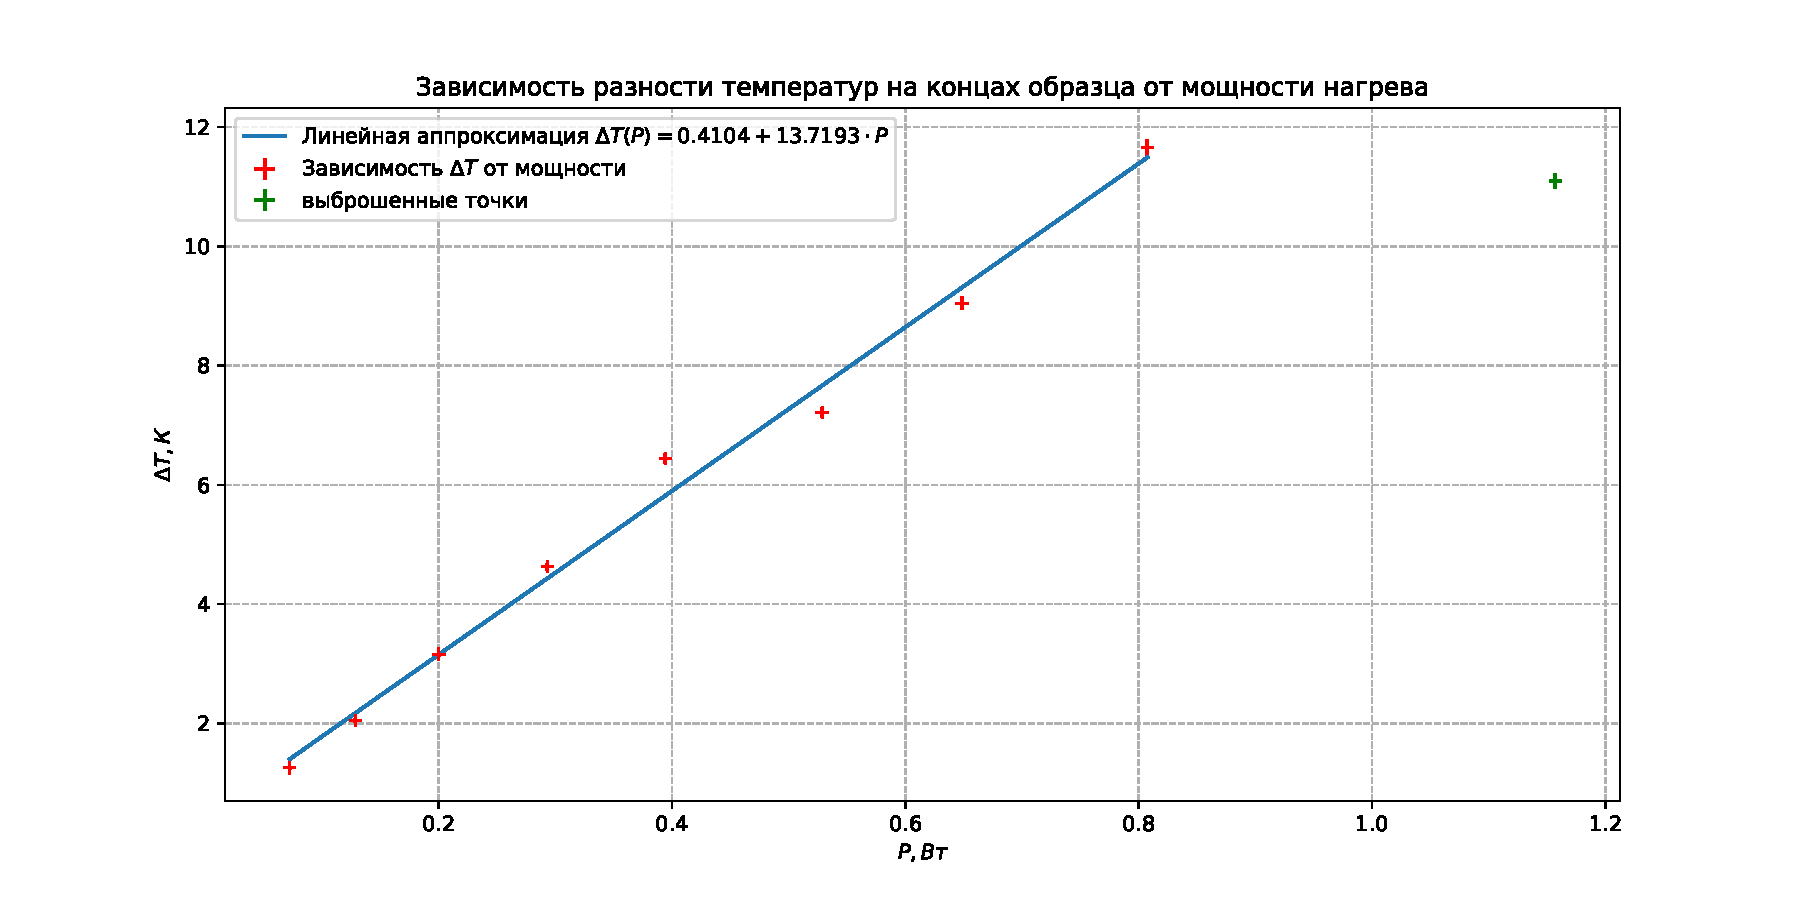
\includegraphics[width=0.8\textwidth]{pictures/DeltaT-P.pdf}
    \caption{Зависимость перепада температур на образце от мощности нагрева}
    \label{pic:deltaT-P}
\end{figure}

\subsection*{Определение постоянной Лоренца}

Температуру эксперимента примем равной комнатной:

\begin{equation}
    T = (300{,}0 \pm 0{,}5)~\text{К}.
\end{equation}

По формуле \eqref{eq:L} получаем

\begin{equation}
    L = (3{,}34 \pm 0{,}13)\cdot 10^{-8}~
    \frac{\text{Вт}\cdot\text{Ом}}{\text{К}^2}.
\end{equation}

Погрешность вычислялась по формуле

\begin{equation}
    \sigma_L = L \sqrt{
        \left(\frac{\sigma_R}{R}\right)^2 +
        \left(\frac{\sigma_A}{A}\right)^2 +
        \left(\frac{\sigma_T}{T}\right)^2
    }.
\end{equation}

Относительно теоретического значения \eqref{eq:L-theory} полученное значение больше примерно на

\begin{equation}
    \frac{L - L_{\text{теор}}}{L_{\text{теор}}} \approx 37\%.
\end{equation}

\subsection*{Оценка удельного сопротивления и теплопроводности}

Исследуемый образец --- алюминий. Для ячейки с алюминием

\begin{equation}
    d = (3{,}50 \pm 0{,}05)~\text{мм}, \qquad
    l = (42{,}0 \pm 0{,}5)~\text{мм}.
\end{equation}

Площадь поперечного сечения:

\begin{equation}
    S = \frac{\pi d^2}{4}, \qquad
    \sigma_S = \frac{\pi d}{2}\sigma_d.
\end{equation}

Получено

\begin{equation}
    S = (9{,}6 \pm 0{,}3)~\text{мм}^2.
\end{equation}

Удельное сопротивление определим из

\begin{equation}
    R = \rho \frac{l}{S}, \qquad
    \rho = \frac{SR}{l}.
\end{equation}

Погрешность:

\begin{equation}
    \sigma_{\rho} = \rho \sqrt{
        \left(\frac{\sigma_l}{l}\right)^2 +
        \left(\frac{\sigma_S}{S}\right)^2 +
        \left(\frac{\sigma_R}{R}\right)^2
    }.
\end{equation}

В результате

\begin{equation}
    \rho = (31{,}5 \pm 1{,}0)\cdot 10^{-8}~\text{Ом}\cdot\text{м}.
\end{equation}

Для коэффициента теплопроводности:

\begin{equation}
    A = \frac{l}{S\kappa}, \qquad
    \kappa = \frac{l}{SA}.
\end{equation}

Погрешность:

\begin{equation}
    \sigma_{\kappa} = \kappa \sqrt{
        \left(\frac{\sigma_l}{l}\right)^2 +
        \left(\frac{\sigma_S}{S}\right)^2 +
        \left(\frac{\sigma_A}{A}\right)^2
    }.
\end{equation}

Получено

\begin{equation}
    \kappa = (32 \pm 2)~\frac{\text{Вт}}{\text{м}\cdot\text{К}}.
\end{equation}

Табличные значения для алюминия при комнатной температуре: $\rho_{\text{табл}} = (2{,}5 \ldots 2{,}7)\cdot 10^{-8}~\text{Ом}\cdot\text{м}$, $\kappa_{\text{табл}} = 220 \ldots 270~\text{Вт}/(\text{м}\cdot\text{К})$. Полученные значения заметно отличаются от табличных, что указывает на существенную систематическую погрешность измерения теплового сопротивления и, возможно, на неидеальность тепловой компенсации экраном.

\subsection*{Оценка времени установления}

Оценим время установления теплового равновесия по формуле

\begin{equation}
    \tau = 3R_{\text{г}}\frac{\rho_{\text{Al}} l^2}{\kappa \mu},
\end{equation}

где $R_{\text{г}}$ --- газовая постоянная, $\rho_{\text{Al}} = 2698~\text{кг}/\text{м}^3$, $\mu = 27\cdot 10^{-3}~\text{кг}/\text{моль}$. Подставляя экспериментальное значение $\kappa$, получаем

\begin{equation}
    \tau \approx 1{,}38 \cdot 10^4~\text{с}.
\end{equation}

Это значение значительно больше характерных времён выдержки в эксперименте, поэтому установление равновесия могло быть неполным. Это согласуется с тем, что одна из точек при малом времени ожидания оказалась выбросом.

\FloatBarrier
\section{Вывод}

\begin{itemize}
    \item Снята ВАХ алюминиевого образца. По линейной аппроксимации получено сопротивление участка образца
    \[
        R = (1{,}376 \pm 0{,}005)\cdot 10^{-4}~\text{Ом}.
    \]

    \item Из зависимости перепада температур от мощности нагрева получено тепловое сопротивление
    \[
        A = (14 \pm 1)~\text{К}/\text{Вт}.
    \]

    \item По результатам измерений определена постоянная Лоренца
    \[
        L = (3{,}34 \pm 0{,}13)\cdot 10^{-8}~
        \frac{\text{Вт}\cdot\text{Ом}}{\text{К}^2}.
    \]
    Она по порядку величины согласуется с теоретическим значением $2{,}44\cdot 10^{-8}~\text{Вт}\cdot\text{Ом}/\text{К}^2$, но превышает его примерно на $37\%$.

    \item Дополнительно получены оценки
    \[
        \rho = (31{,}5 \pm 1{,}0)\cdot 10^{-8}~\text{Ом}\cdot\text{м}, \qquad
        \kappa = (32 \pm 2)~\frac{\text{Вт}}{\text{м}\cdot\text{К}}.
    \]
\end{itemize}

Основной источник расхождения с табличными значениями, вероятно, связан с измерением теплопроводности: неполное установление теплового равновесия, остаточный теплообмен с экраном и завышение мощности из-за падения напряжения на подводящих проводах.

\end{document}
